\documentclass[12pt, a4paper]{article}
\usepackage{babel}
\usepackage{cleveref}
\usepackage{graphicx}

% Setter mindre marginer for å få mer plass
\usepackage[margin=2.5cm]{geometry}

% Pakke for å ha tekst rundt figurer
\usepackage{wrapfig}

% Pakke for å ha figurer side om side
\usepackage{subcaption}

% Kommando som gjør at bilder kan være i en mappe som heter "bilder"
\graphicspath{ {./bilder/} }

% Må ha for referanselista
\usepackage{url}




\title{
    Project \#1\\
    \large Plastic Scanner Initial Checks\\
}
\author{
    Stein Lysberg
}


\begin{document}

    
    \maketitle
    \tableofcontents
    \thispagestyle{empty}
    \addtocounter{page}{-1}
    \clearpage

    \section{Introduction}

    
        This report is the first in a series of five, about the use of a Nordic Semiconductor
        nRF52 Development Kit (nRF52 DK) along with a Printed Circuit Board (PCB) for scanning plastics.
        The PCB is designed for use with an Arduino Uno rev. 3 \cite{DB23}. This report
        will investigate wether the PCB is built according to given specifications, as well as
        whether the nRF52 DK and PCB are compatible with one another.

        \subsection{Verification of component placement}
            \begin{wrapfigure}[11]{r}{0.35\textwidth}
                \centering
                \vspace{-100pt}
                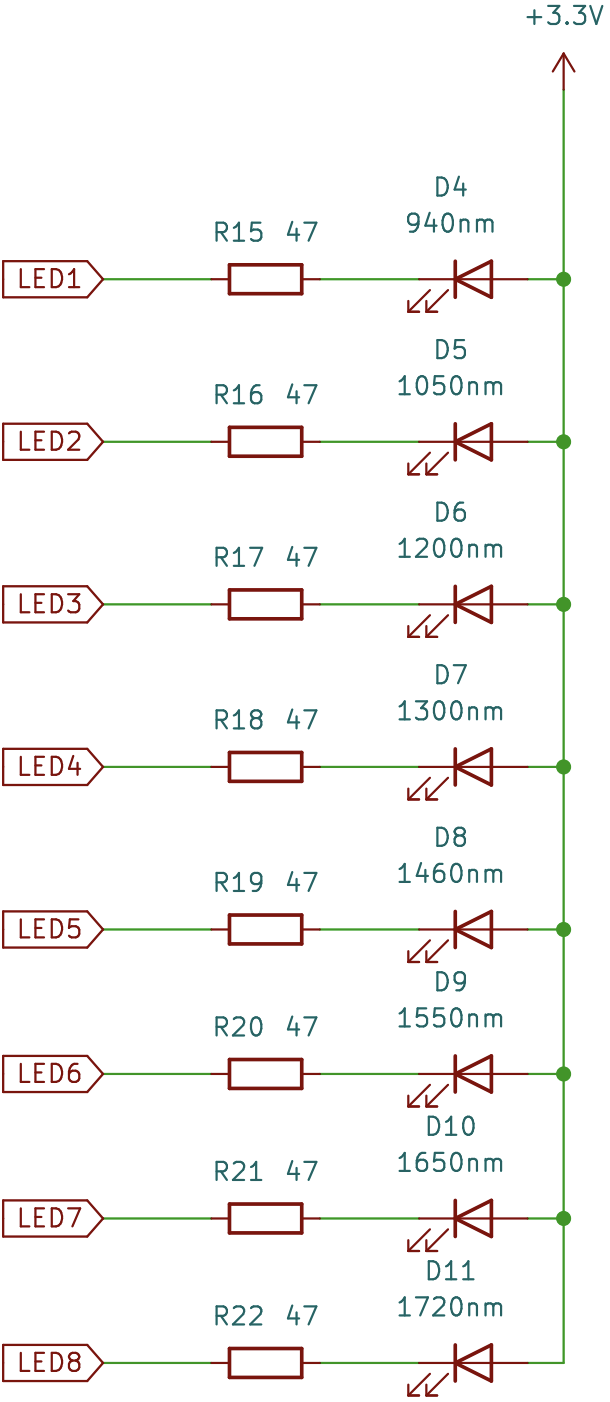
\includegraphics[width=0.28\textwidth]{ledschematic.png}
                \caption{LED schematic \cite{DB23}.}
                \label{fig:ledschematic}
            \end{wrapfigure}

            \begin{minipage}{0.6\textwidth}
                \vspace{0pt}
                This section will look at wether or not components are correctly placed on the PCB. In summary:
                \begin{itemize}
                    \item D1-D5, D12 are all present and correctly placed on the PCB. 
                    \item D10, D11 are missing as mentioned in BOM. 
                    \item U1-U4 are all present and correctly placed on the PCB. 
                    \item No component is misplaced or incorrectly  soldered.
                \end{itemize}
                This will be explained further, starting with the placement of diodes.
                \vspace{-10pt}
                \noindent  
            \end{minipage}


            \subsubsection{Placement of diodes}


    

            
                \noindent \Cref{fig:ledschematic} 
                shows how the LEDs should be mounted on the PCB, 
                indicating what is the correct orientation when mounted. Note 
                that all LEDs are connected to the same node.
                \Cref{fig:ledring} shows how the LEDs are mounted. Note that the
                markings, as indicated by the blue arrows, are on the cathode for D4 and D5,
                and on the anode for D6-D9. This is shown in \cref{fig:ledmanual}, which contains excerpts
                from the user manuals for these LEDs.
                It also shows that D10 and D11 is 
                missing, which is in accordance with the bill of materials.

                \begin{figure}[h!]
                    \centering
                    \vspace{0pt}
                    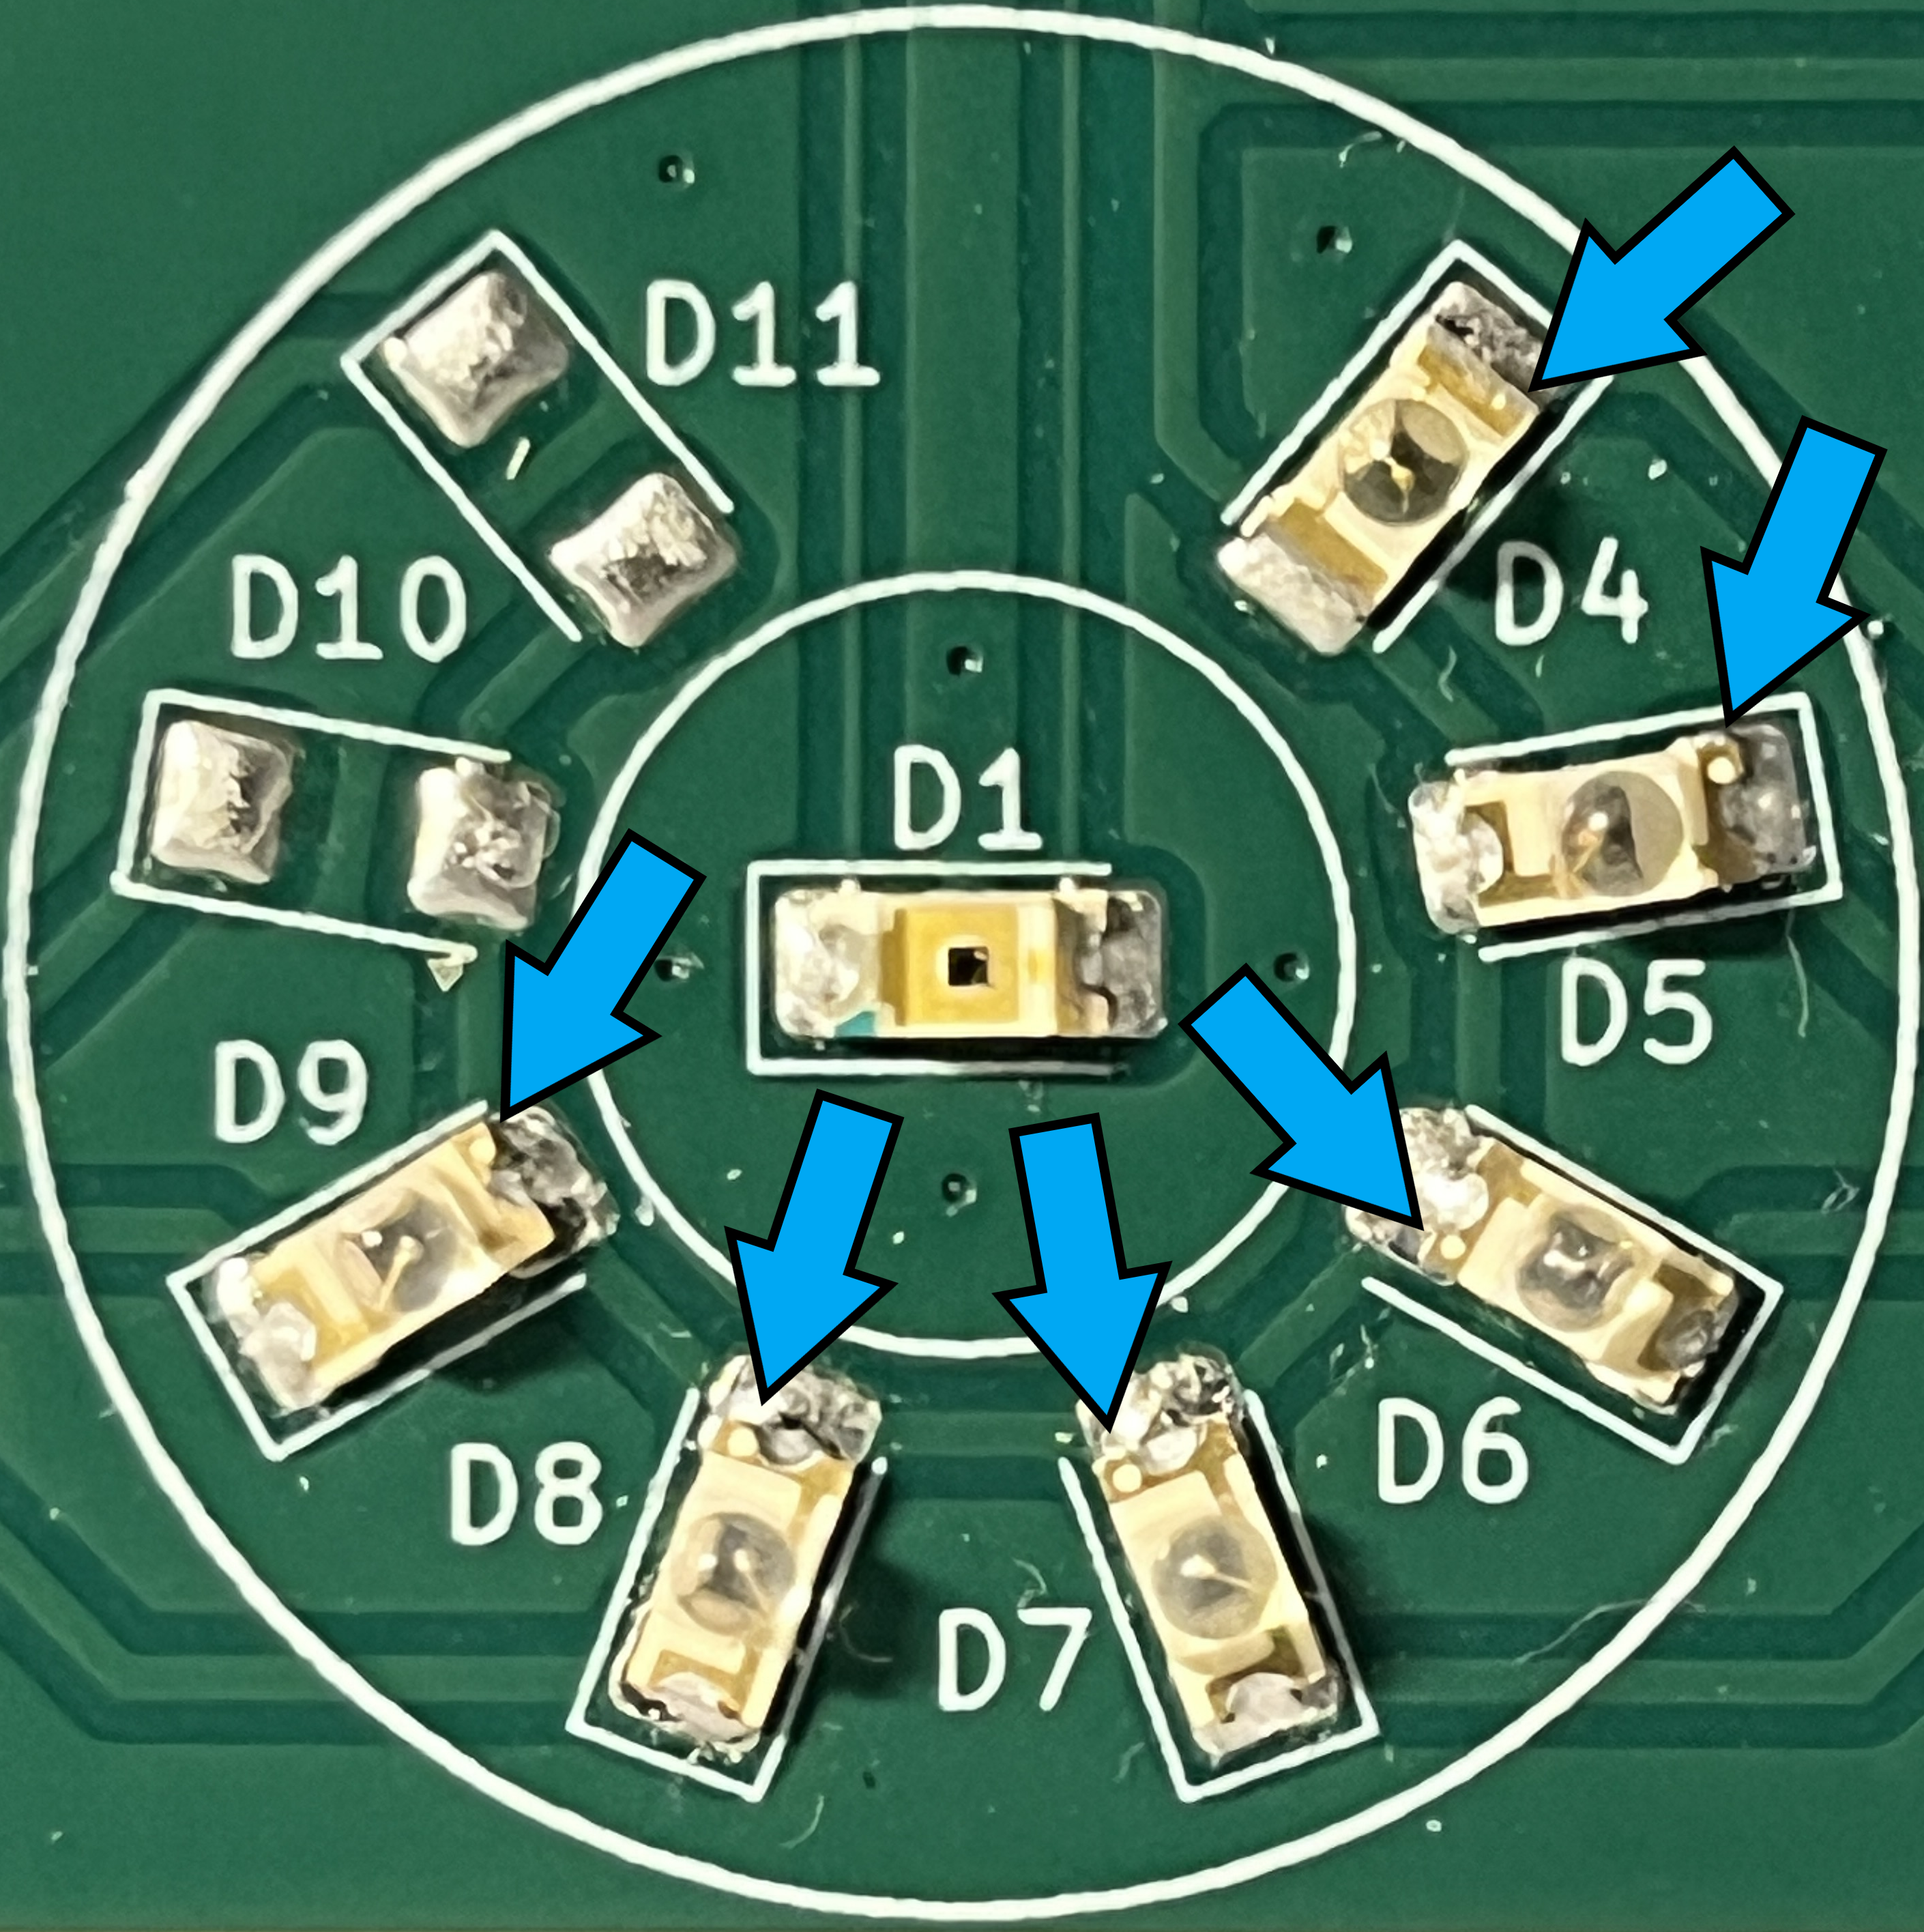
\includegraphics[width=0.30\textwidth]{ledring.png}
                    \caption{LEDs on the board.}
                    \label{fig:ledring}
                \end{figure}

                \begin{figure}[h!]
                \begin{subfigure}[t]{\textwidth}
                    \centering
                    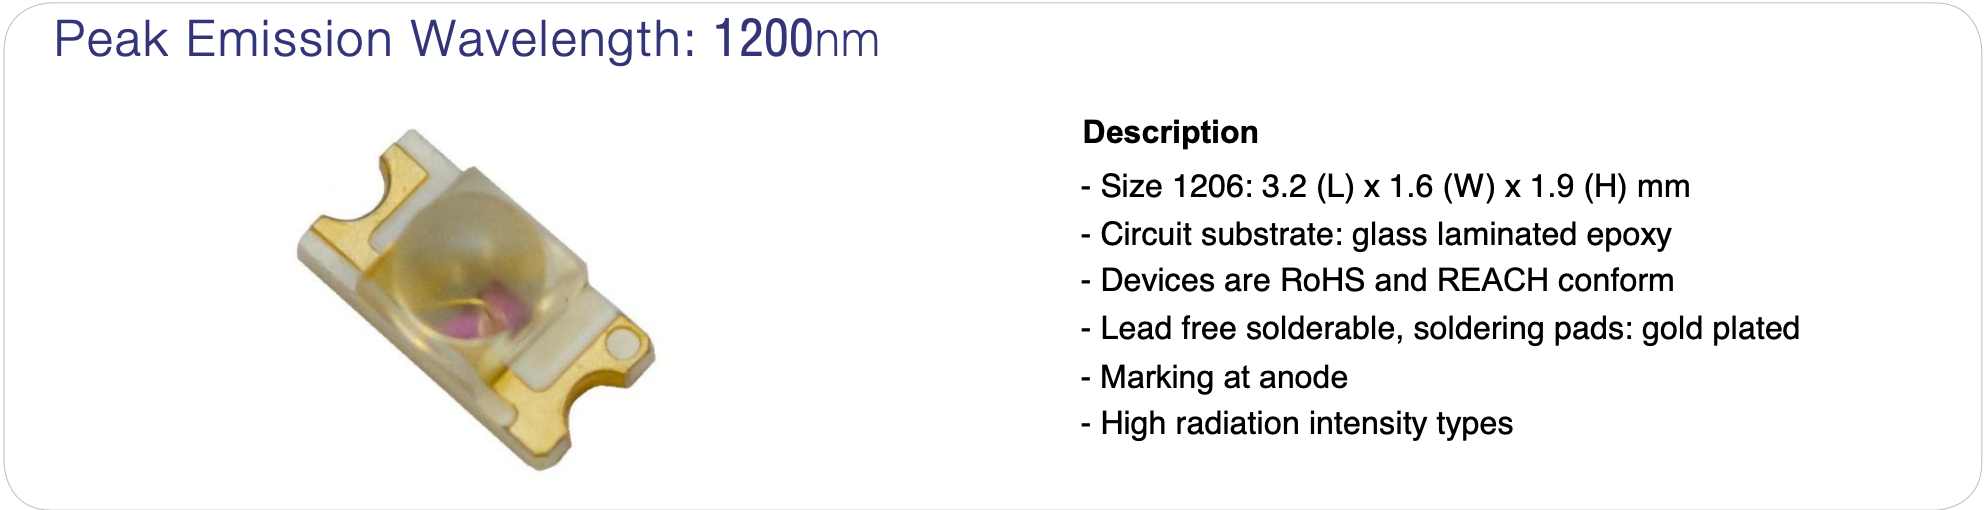
\includegraphics[width=0.8\textwidth]{led6.png}
                    \label{fig:D6}
                    \caption{D6}
                \end{subfigure}
                \begin{subfigure}[t]{\textwidth}
                    \centering
                    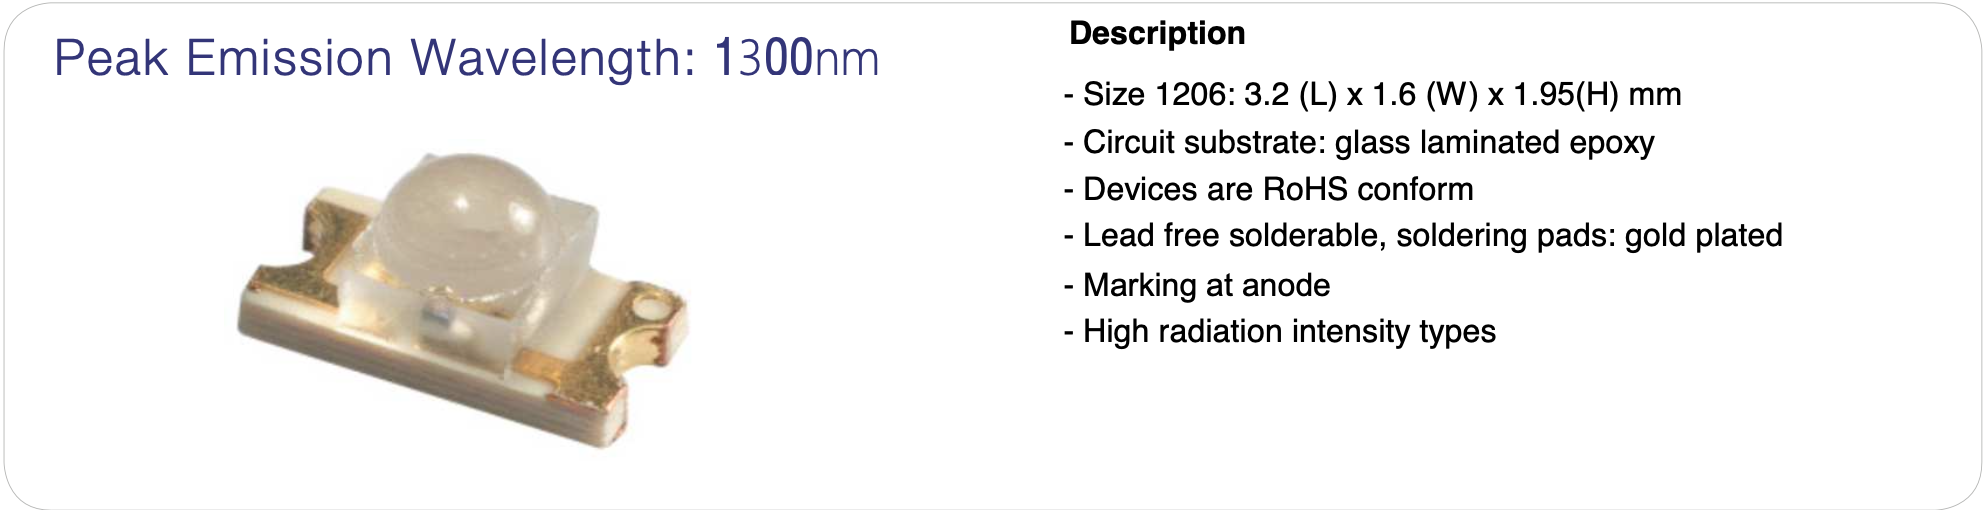
\includegraphics[width=0.8\textwidth]{led7.png}
                    \label{fig:D7}
                    \caption{D7}
                \end{subfigure}
                \begin{subfigure}[t]{\textwidth}
                    \centering
                    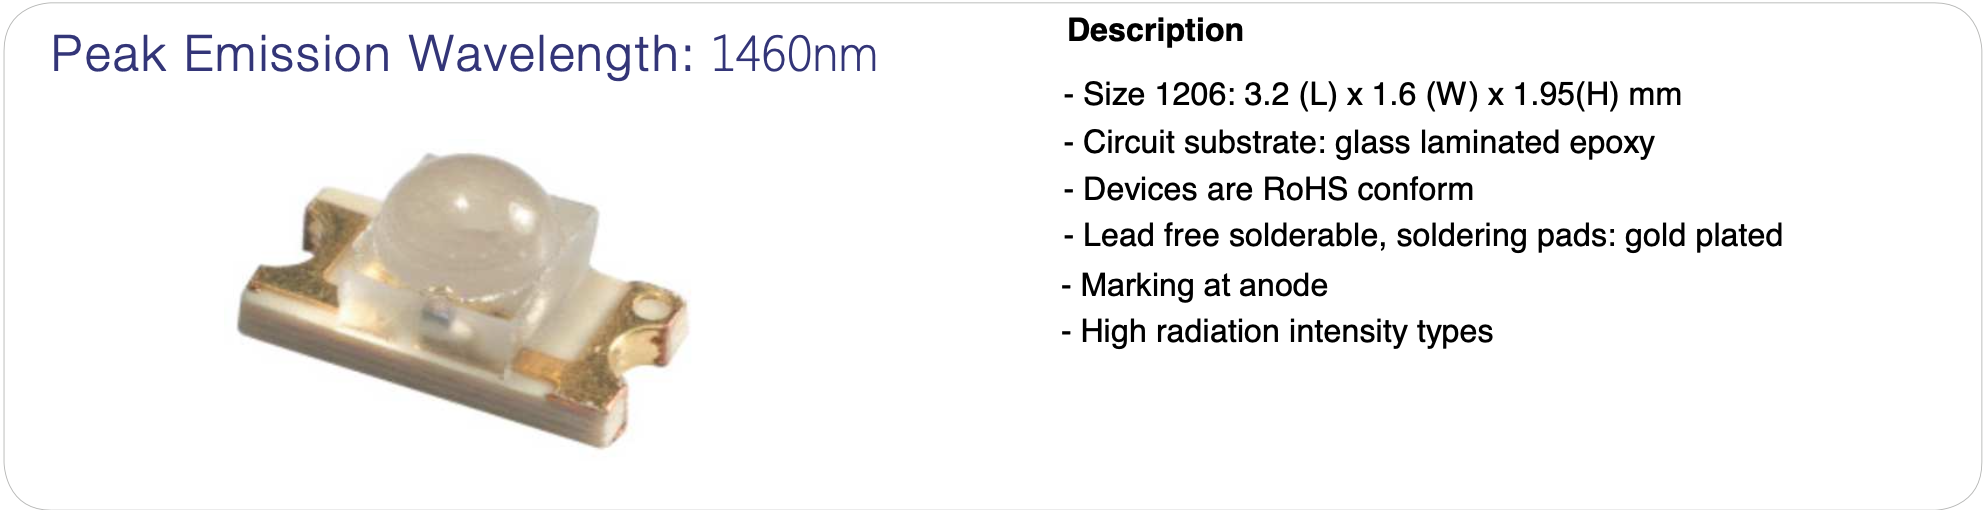
\includegraphics[width=0.8\textwidth]{led8.png}
                    \label{fig:D8}
                    \caption{D8}
                \end{subfigure}
                \begin{subfigure}[t]{\textwidth}
                    \centering
                    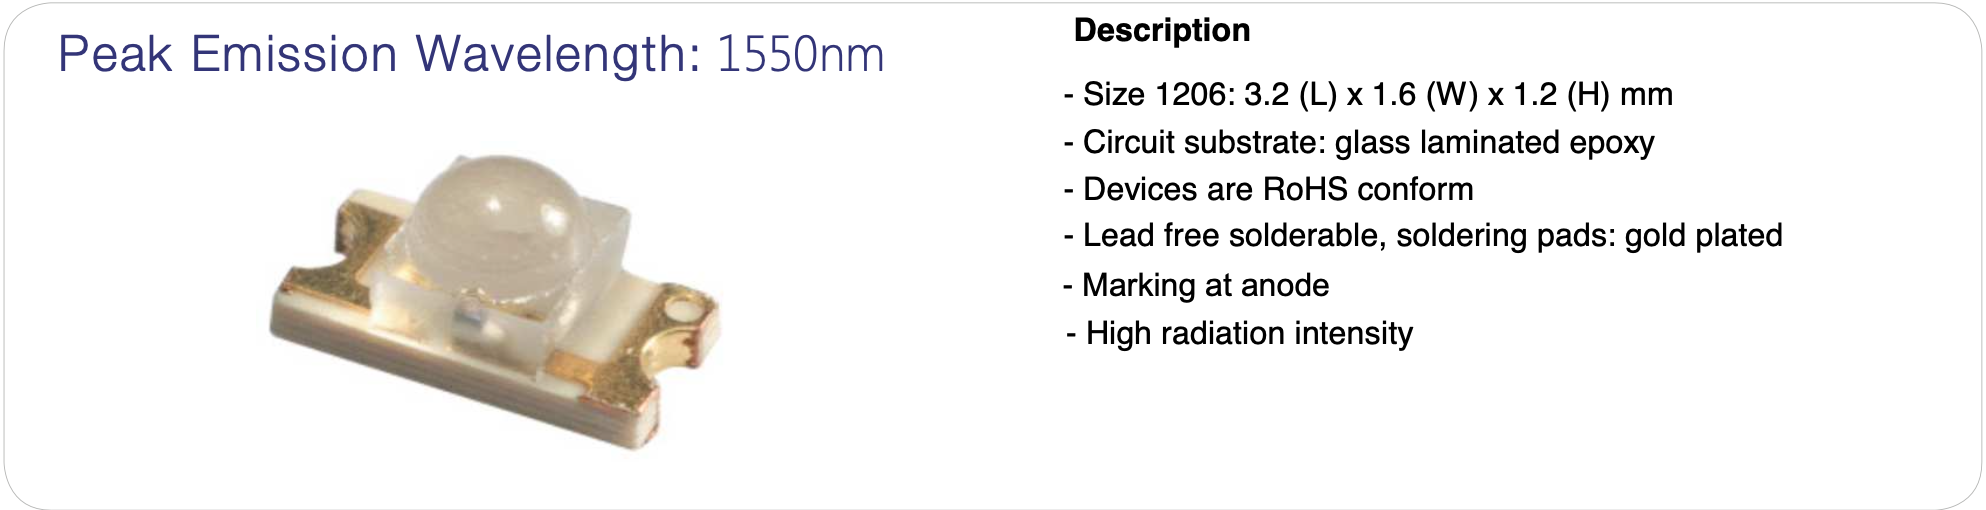
\includegraphics[width=0.8\textwidth]{led9.png}
                    \label{fig:D9}
                    \caption{D9}
                \end{subfigure}
                \caption{LED documentation stating markings are at anode \cite{led6, led7, led8, led9}.}
                \label{fig:ledmanual}
                \vspace{0pt}
            \end{figure}
            \clearpage

            \subsubsection{Placement of chips}
        The chips are also correctly mounted, as indicated by the orientation marks. \Cref{fig:chipexamples} shows this.

        \begin{figure}[h!]
                \begin{subfigure}[t]{0.33\textwidth}
                    \centering
                    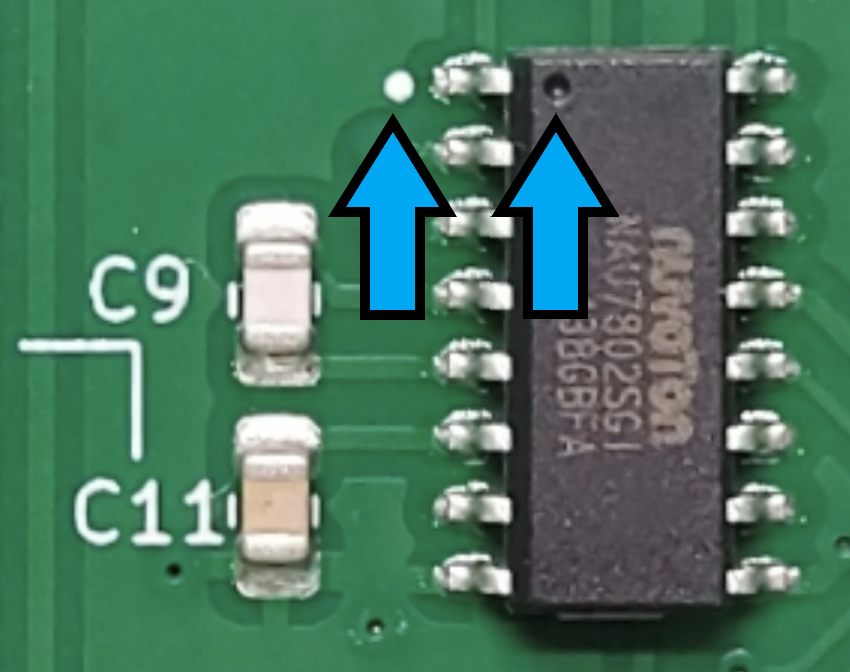
\includegraphics[width=0.8\textwidth]{chip1.png}
                    \label{fig:chip1}
                \end{subfigure}%
                \begin{subfigure}[t]{0.33\textwidth}
                    \centering
                    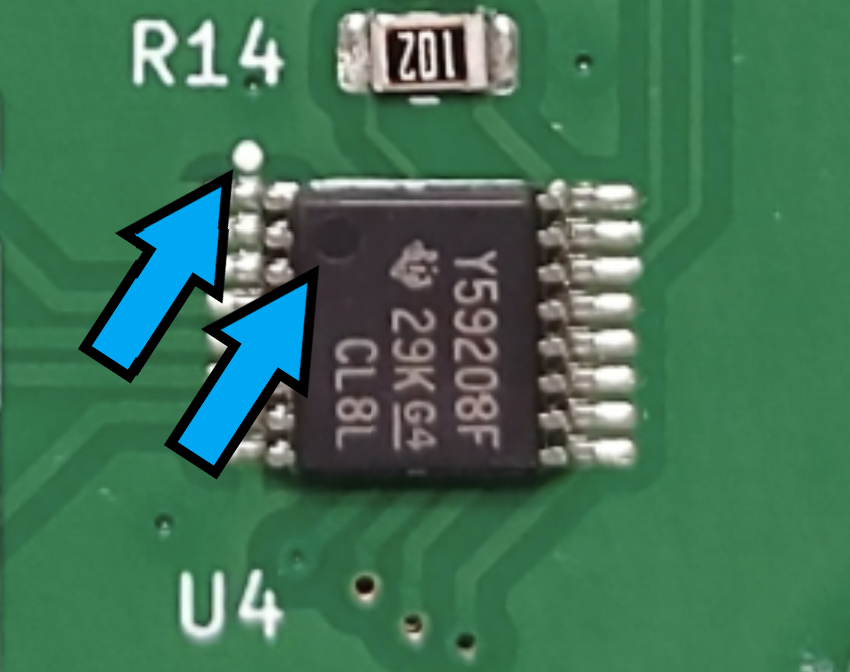
\includegraphics[width=0.8\textwidth]{chip2.png}
                    \label{fig:chip2}
                \end{subfigure}%
                \begin{subfigure}[t]{0.33\textwidth}
                    \centering
                    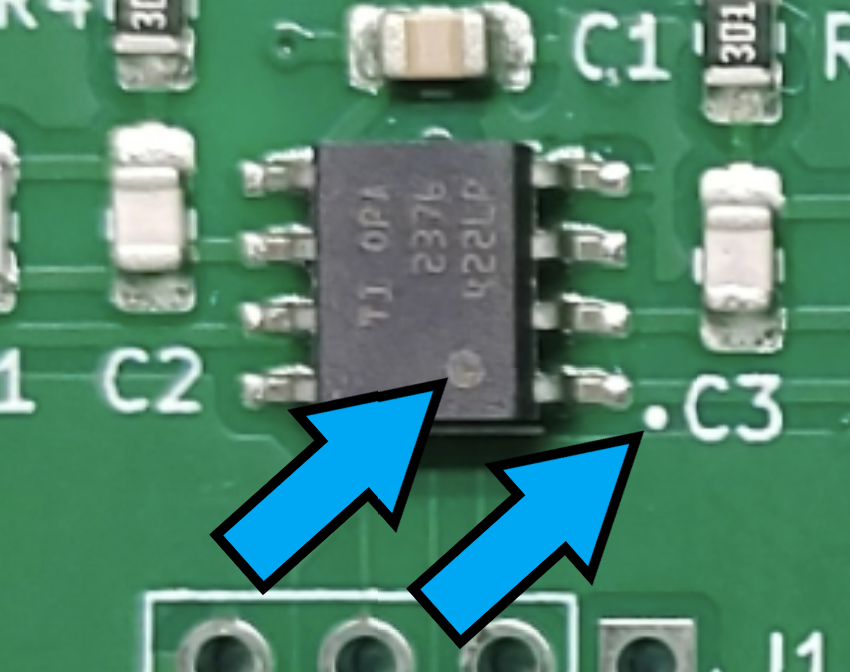
\includegraphics[width=0.8\textwidth]{chip3.png}
                    \label{fig:chip3}
                \end{subfigure}
                \caption{Chips on the PCB.}
                \label{fig:chipexamples}
                \vspace{0pt}
            \end{figure}


        \subsection{Compatability analysis}
            \begin{wrapfigure}[8]{r}{0.50\textwidth}
                    \centering
                    \vspace{-40pt}
                    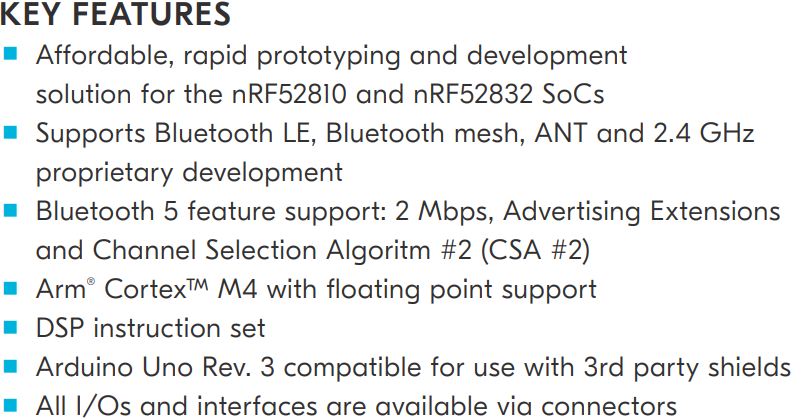
\includegraphics[width=0.45\textwidth]{compatability.png}
                    \caption{Key features of nRF52 DK \cite{nrf52brief}.}
                    \label{fig:compatability}
                \end{wrapfigure}
            As shown in \cref{fig:compatability}, the nRF52 DK should be compatible with 3rd party
            Arduino shields. The plastic scanner PCB is such a shield, and it follows that the nRF52 DK
            can replace the Arduino Uno Rev. 3 in the plastic scanner. The compatability will however be
            investigated a bit further.
            
            \subsubsection{Absolute maximum ratings}

            \begin{figure}[h!]
                    \centering
                    \vspace{10pt}
                    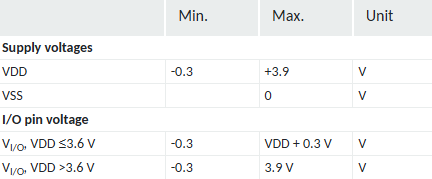
\includegraphics[width=0.6\textwidth]{absmax.png}
                    \caption{Absolute maximum ratings for the nRF52832 \cite{nrf52spec}.}
                    \label{fig:absmax}
                \end{figure}
            
                \noindent \Cref{fig:absmax} shows the absolute maximum ratings for the nRF52 DK IO pins to be
                3.9V. The plastic scanner is built for 5V input, but as \cref{fig:5to3v} shows, the 5V input is
                adjusted down to 3.3V, which is within the absolute maximum ratings.

                \begin{figure}[h!]
                    \centering
                    \vspace{10pt}
                    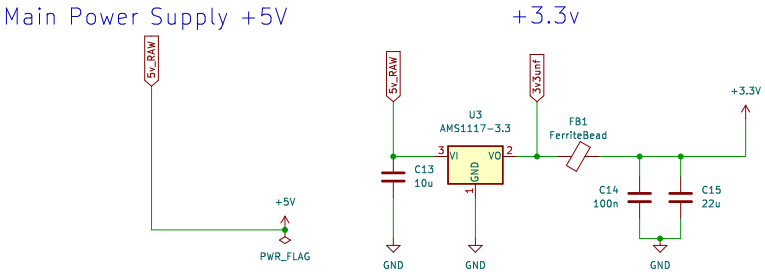
\includegraphics[width=0.65\textwidth]{5to3v.png}
                    \caption{Plastic scanner power supply \cite{DB23}.}
                    \label{fig:5to3v}
                \end{figure}

            \subsubsection{Logic voltage}

                \begin{figure}[h!]
                    \centering
                    \vspace{10pt}
                    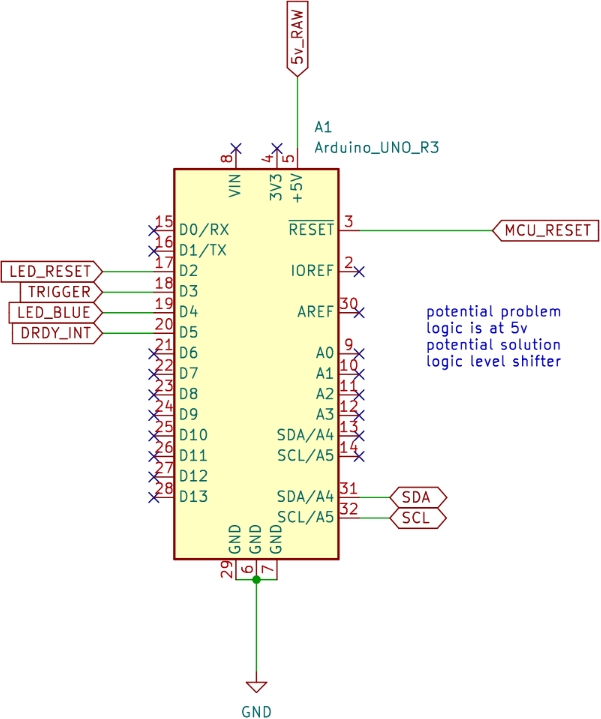
\includegraphics[width=0.55\textwidth]{voltagelevel.png}
                    \caption{Arduino schematic \cite{DB23}.}
                    \label{fig:voltagelevel}
                \end{figure}
            
            \Cref{fig:voltagelevel} shows a warning (blue text) about the logic voltage for the Arduino
            being at 5V, which further indicates that a lower voltage is preferable for the plastic scanner.
            As shown in \cref{fig:buttons}, the MCU\_RESET and TRIGGER are both pulled up to 
            the 5V raw flag when buttons are inactive, which is at 5V when the development board is 
            connected to the USB port. This is a potential issue as the voltage exceeds the nRF52 DK 
            I/O pin max voltage of 3.9V.

                \begin{figure}[h!]
                    \centering
                    \vspace{10pt}
                    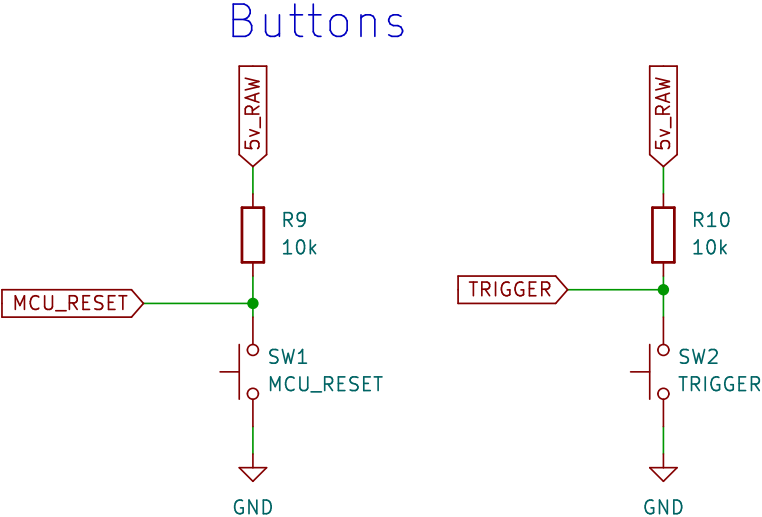
\includegraphics[width=0.35\textwidth]{buttons.png}
                    \caption{Arduino schematic \cite{DB23}.}
                    \label{fig:buttons}
                \end{figure}

    \clearpage
    \section{Discussion}
            
            \subsection{Markings on LEDs}

                LEDs are commonly marked on the cathode, however in the case of D6-D9 the markings are on the anode.
                The PCB was originally soldered based on the assumption that markings would be on the cathode, and so
                they had to be re-soldered. This is shown in \cref{fig:beforeandafter}.  

            \begin{figure}[h!]
                \begin{subfigure}[t]{0.5\textwidth}
                    \centering
                    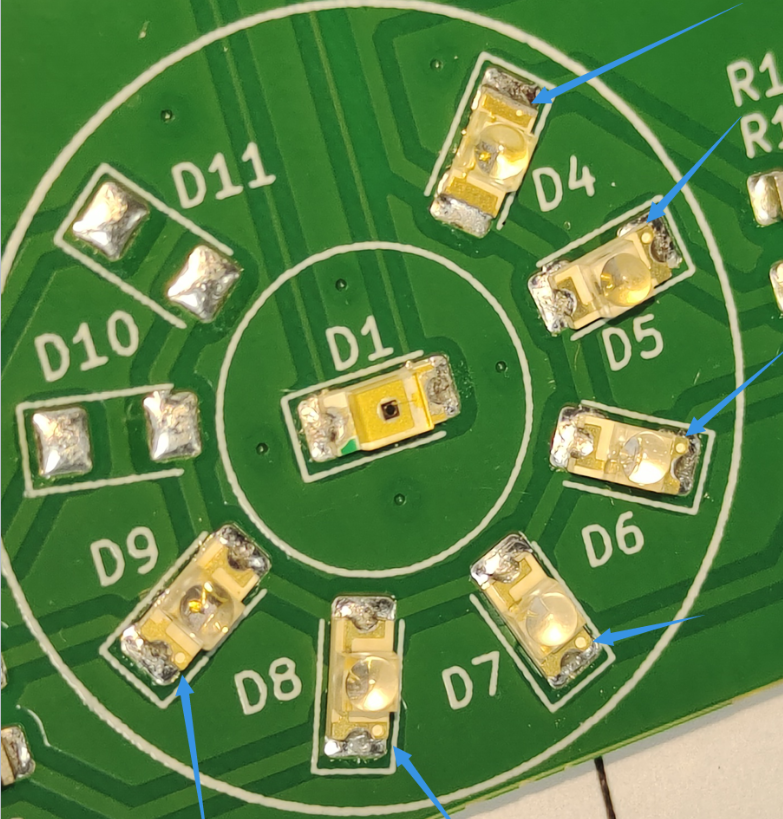
\includegraphics[width=0.77\textwidth]{ledsbefore.png}
                    \caption{Before.}
                    \label{fig:before}
                \end{subfigure}%
                \begin{subfigure}[t]{0.5\textwidth}
                    \centering
                    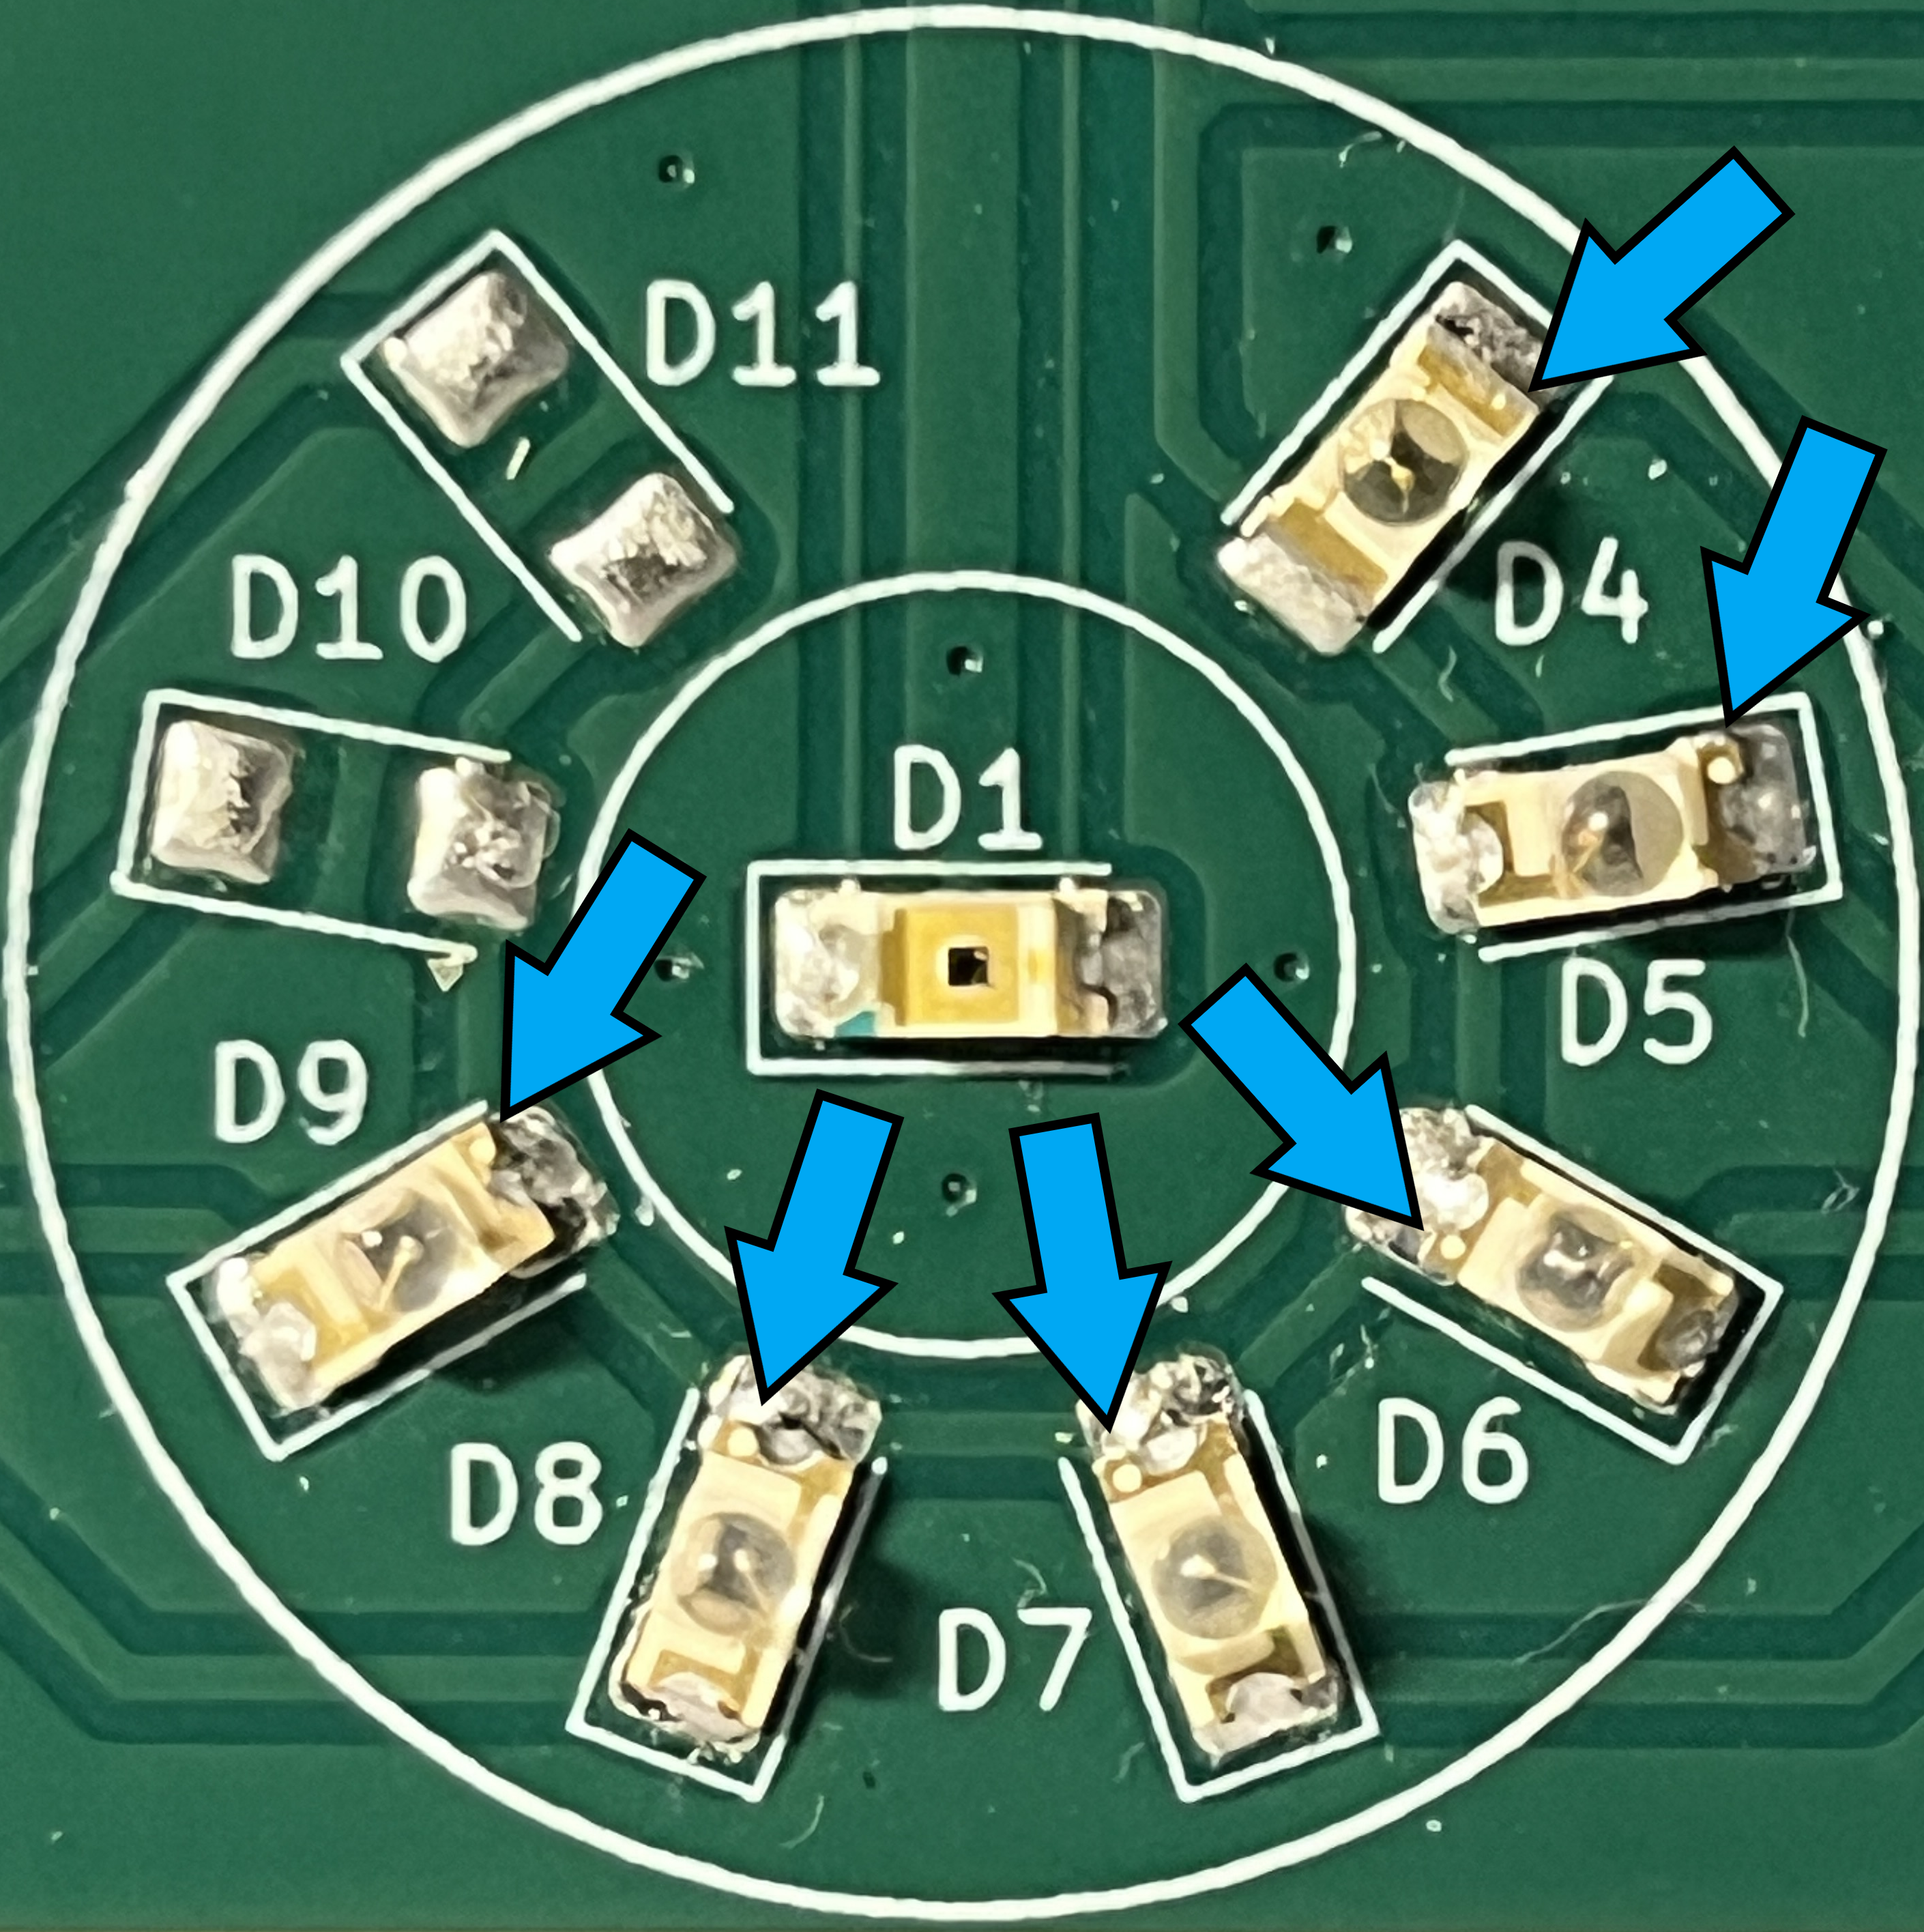
\includegraphics[width=0.8\textwidth]{ledring.png}
                    \caption{After}
                    \label{fig:after}
                \end{subfigure}%
                \caption{LEDs before and after resoldering.}
                \label{fig:beforeandafter}
                \vspace{0pt}
            \end{figure}

            \subsection{Logic at 5V}

                As stated above, MCU\_RESET and TRIGGER are pulled up to the 5V raw flag, which is an issue
                as the voltage exceeds the nRF52832 I/O pin
                max voltage of 3.9V. A voltage divider can be used to reduce the voltage to 3.3V, 
                but it would require some changes to the PCB design. Another option, and the one that
                will be practiced, is to simply ignore the issue and use it as it is.


            
    \section{Conclusion}
                The plastic scanner was not built correctly according to spec initially, because four of
                the LEDs were soldered the wrong way around. However after re-soldering, it is built correctly.
                The nRF52 DK and the plastic scanner are not compatible on paper, due to MCU\_RESET and TRIGGER
                exceeding the maximum I/O voltage for the nRF52832. This issue will be overlooked, and the plastic
                scanner will be used with the nRF52 DK. 

    \clearpage
    \addcontentsline{toc}{section}{References}  
    \bibliographystyle{IEEEtran}
    \bibliography{bibliography}

\end{document}